\chapter{Verilog e RTL}

Gli RTL, o Register Transfer Language, permettono di descrivere cosa succede a livello di circuito fra registri. Vengono utilizzati per descrivere l'hardware. Vedremo il linguaggio \textbf{Verilog}. Gli RTL permettono di descrivere e comporre dei moduli. Il libro di testo propone il dialetto \textbf{System Verilog} che mette a disposizione due metodi per descrivere i moduli. Un metodo è il metodo \textit{constructive}, noi vedremo il metodo \textit{behavioral} dove ad esempio un Multiplexer da 2 vie 1 bit è descritto da:
\begin{lstlisting}[style={verilog}]
	z = (ic == 0 ? x : y)
\end{lstlisting}

Verilog è un linguaggio compilato. Un file System Verilog compilato produce una traccia di esecuzione e un eseguibile che simula il comportamento dei moduli. Viene detta \textbf{simulazione}.

Un programma Verilog può anche essere dato in input a un programma detto \textbf{synthetizer}, che produce una \textbf{netlist}, ovvero una lista dei componenti e dei collegamenti per realizzare il modulo fisicamente. Un altro modo per realizzare la sintesi è utilizzare un \textbf{FPGA}, o Field-programmable gate array. Un FPGA è un circuito integrato composto da una matrice di celle, e una singola cella può:
\begin{enumerate}
	\item Eseguire una funzione booleana di 3-5 ingressi con 1 uscita 
	\item Implementare un bit di memoria
	\item Routing
\end{enumerate} 

Un FPGA moderno comprende, oltre a delle celle, delle righe che contengono diversi componenti come delle ALU.

\begin{figure}[H]
	\centering
	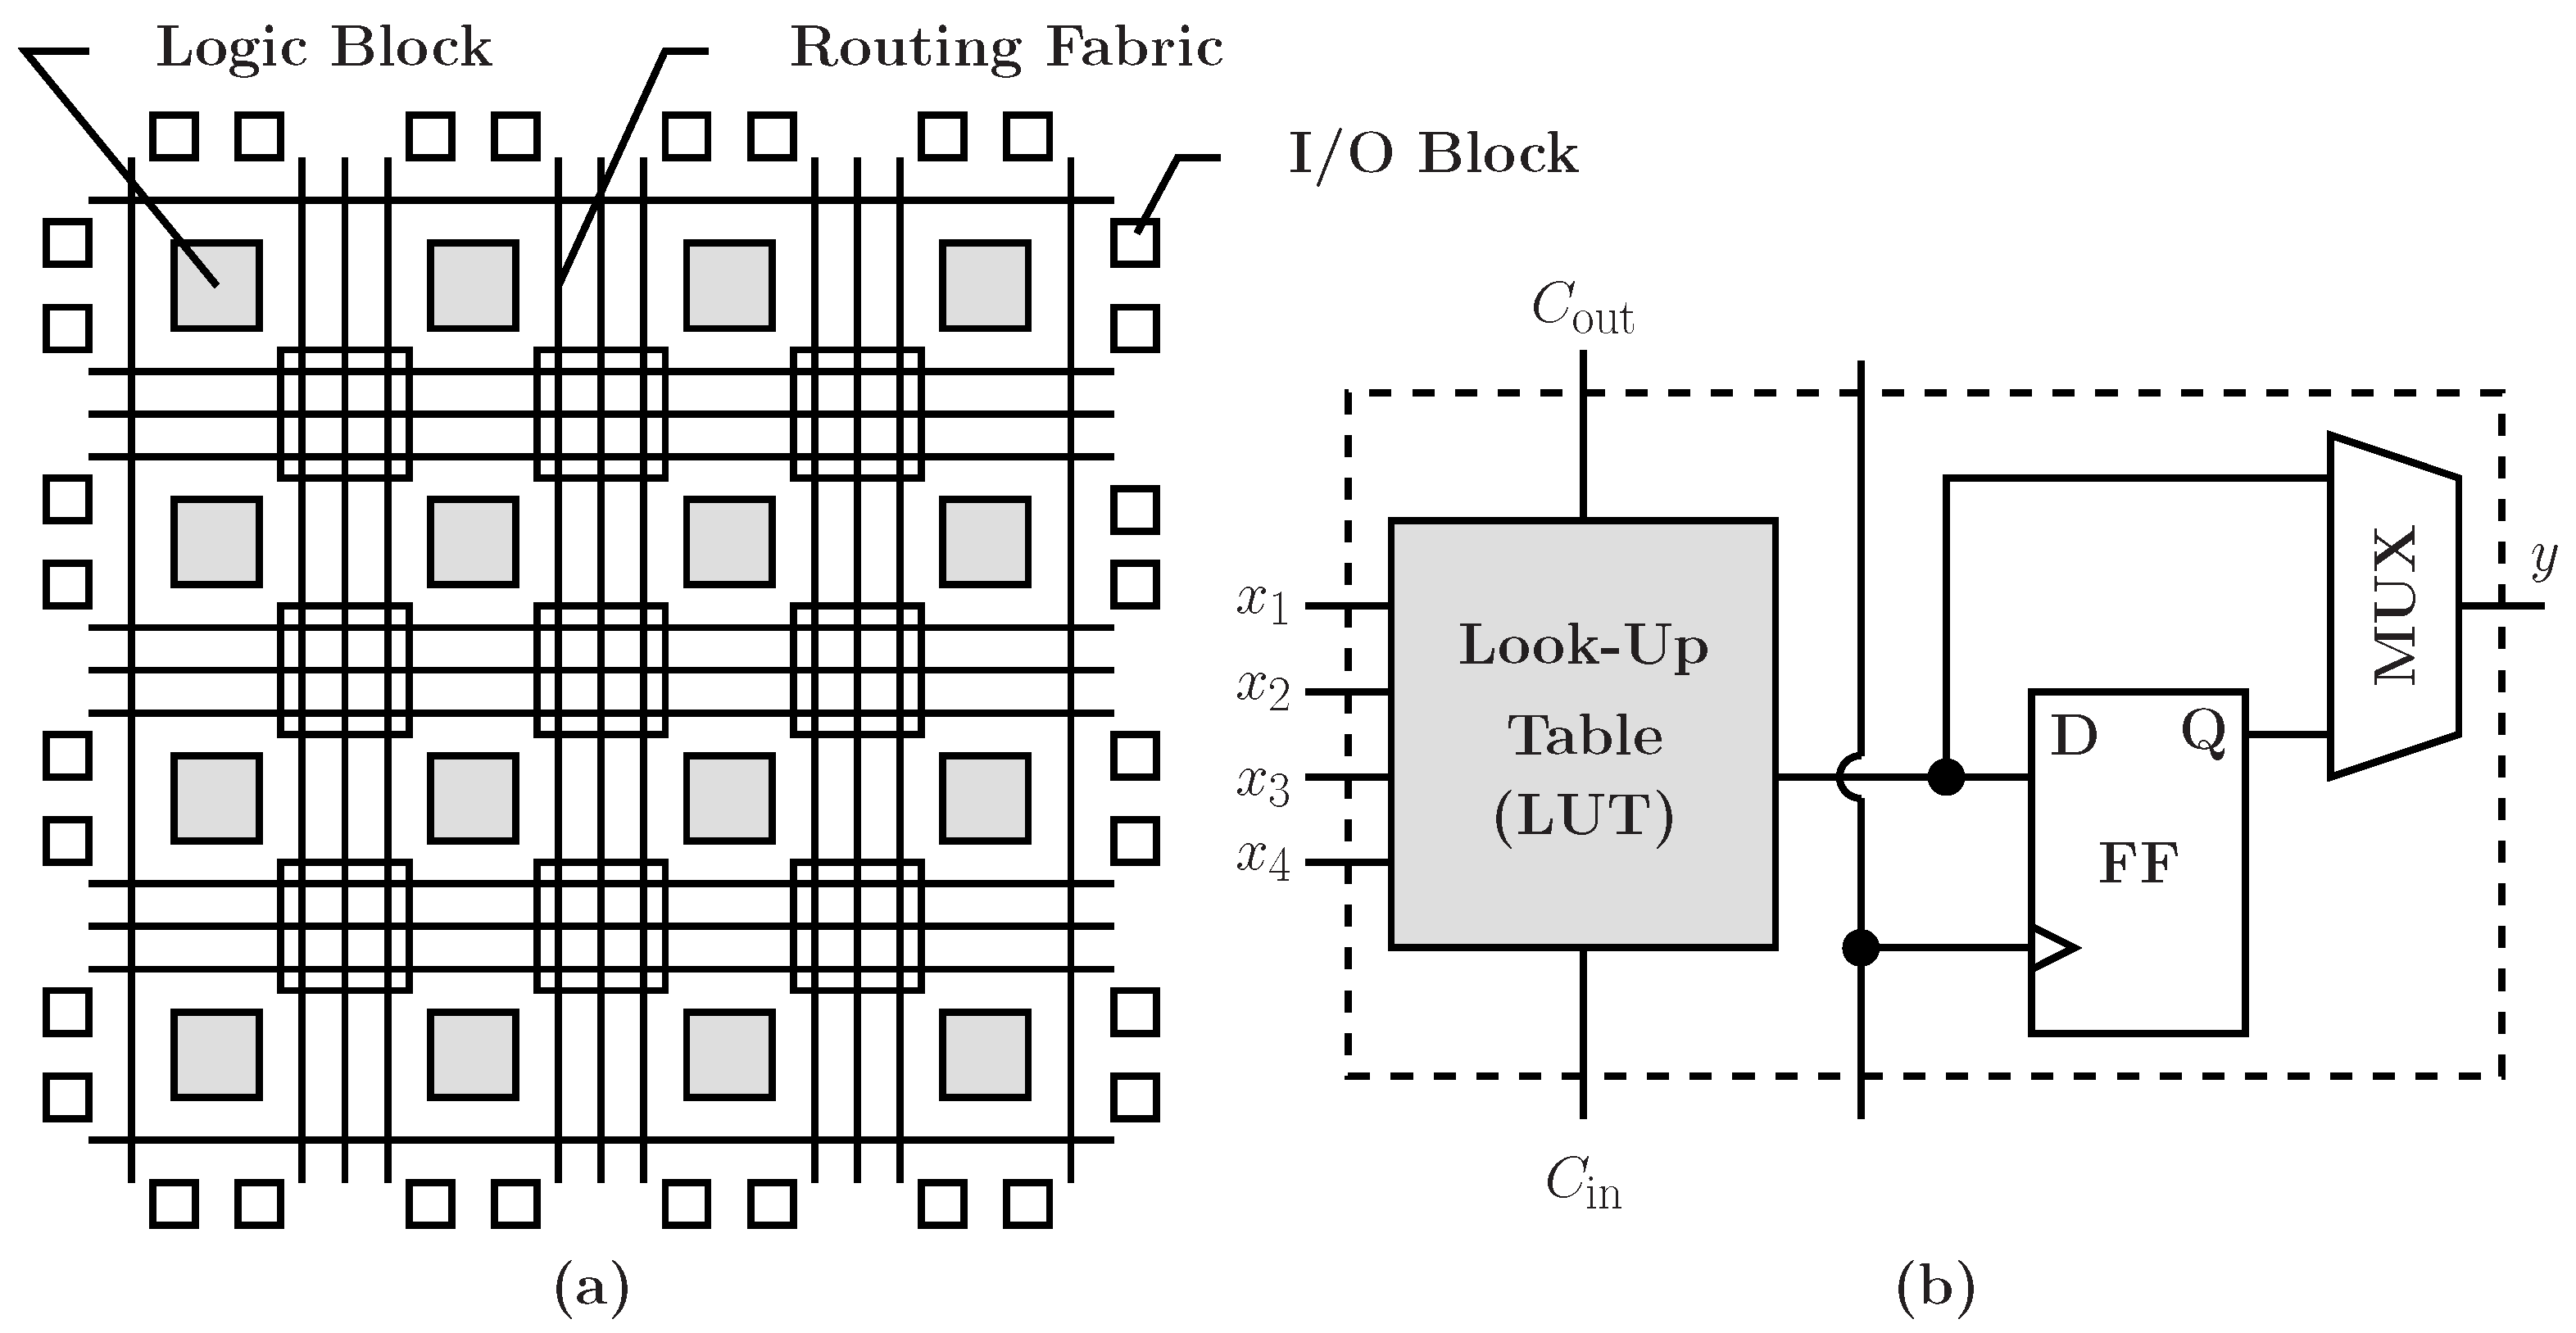
\includegraphics[]{fpga1}
	\caption{Schema FPGA}
\end{figure}

\section{Scrivere e compilare System Verilog}

Creiamo un multiplexer da due bit con System Verilog, compiliamo e visualizziamo con \textbf{GTKWave}

\includecode[verilog]{./verilog/2x1mux/mux.sv}{mux.sv}
\includecode[verilog]{./verilog/2x1mux/test_mux.sv}{test\_mux.sv}

Per compilare, eseguiamo da terminale 
\begin{lstlisting}[style={bash}]
iverilog -g2005-sv nome_sorgente.sv -o nome_eseguibile
\end{lstlisting}

Quindi, per compilare entrambi i file e caricarli in GTKWave:
\begin{lstlisting}[style={bash}]
iverilog -g2005-sv test_mux.sv mux.sv -o test_mux
# Eseguiamo la simulazione
./test_mux
# Viene creato il file provamux.vcd, carichiamolo in GTKWave
gtkwave provamux.vcd &
\end{lstlisting}

\includecode[verilog]{./verilog/2x1mux/mux4.sv}{Multiplexer da 4 vie ad 1 bit}

\includecode[verilog]{./verilog/2x1mux/muxbool.sv}{Multiplexer di variabili booleane}

\clearpage

\section{Esercizi}

\paragraph{Automa di Mealy per riconoscere "abba"}
Abbiamo visto nella sezione precedente un automa di Mealy a stati finiti per riconoscere una stringa "abba" in un una stringa nell'alfabeto $ \{a,b,c\} $.
Abbiamo 3 moduli. Uno per il registro, uno per il modulo $ \omega $ e uno per il modulo $ \sigma $. Scriviamolo in Verilog.

% TODO finisci automa in verilog.

\includecode[verilog]{./verilog/abbamealy/register.v}{Registro a N bit}
\includecode[verilog]{./verilog/abbamealy/sigma.v}{Modulo di $ \sigma $}
\includecode[verilog]{./verilog/abbamealy/omega.v}{Modulo di $ \omega $}
\includecode[verilog]{./verilog/abbamealy/abba.v}{Modulo della rete sequenziale}